To this date, sustainable energy sources have become an area in focus worldwide in an attempt to reduce the environmental impact due to emissions of CO2 and other greenhouse gasses. The development of competitive systems to exploit renewable energy sources is the best alternative to reduce the use of fossil fuels for the production of electricity. Over the last years there have been a considerable increase in electricity production from renewable energy sources being the fastest growing sector wind and solar energy. In 2017, solar photovoltaic was the renewable energy source which experienced the highest increased in newly installed capacity amounting a total installed capacity of approximately 402 GW.[ref] %[http://www.ren21.net/wp-content/uploads/2018/06/17-8652_GSR2018_FullReport_web_-1.pdf] 

Photovoltaic (PV) is referred to the production of electricity in the form of direct current (DC) directly from sunlight shining on solar cells. Solar cells are semiconductor devices which typically can produce around 0.5 V DC so they are series connected to form a PV module/panel which can also be connected to other PV panels resulting in a PV array. This way, according to the system´s requirements, the PV panels can be interconnected in series or parallel in order to get at the output a higher voltage or current, respectively. Connecting PV panels either in series or parallel will result in an increase of the system´s overall electricity production.  %[http://www.sabz-energy.com/solar%20electricity%20handbook%202017.pdf] 

Nevertheless, it is essential to keep into consideration the mismatches that may appear between the power generated by the different PV panels, which will result in losses in the PV system and thus in a lower efficiency. Mismatches occur when the PV modules operate in a different operating point than its maximum power point (MPP) due to partial shading, manufacturing tolerances, defects in the PV modules due to weather conditions and aging, among others. Even a small mismatch in one of the PV modules can result in a very high reduction of the power production from the entire PV array. Mismatch losses in a PV system can be reduced by forcing every PV module to work at its MPP by using a technique known as Maximum Power Point Tracking (MPPT). This can be reached by using electronic devices called Module Integrated Converters (MICs) which basically consist on DC-AC micro inverters or DC-DC converters that incorporate a MPPT unit to ensure that the output power of the MIC is the one corresponding to the MPP of the PV module.%[https://www.researchgate.net/publication/43248773_Study_on_MPP_mismatch_losses_in_photovoltaic_applications] 

This project focuses on the design and test of a MIC based on a non-inverting buck-boost DC/DC converter for integration with a PV module in order to operate at its MPP and thus harvest maximum energy from the sunlight. 

\section{PV generation}

The phenomenon on which the transformation of solar energy to electrical energy is based is known as the \textit{Photovoltaic effect}. This phenomenon was first discovered by a French physicist named Edmond Becquerel in 1839 and is based on the emission, from the sunlight or light, of massless photons which collate on two superimposed layers of semiconductor material causing some of the electrons to flow and, hence, allowing the generation of voltage and electric current. Solar PV cells are made of a negative charged layer (n-layer) and a positive charged layer (p-layer) of a semiconductor material, usually crystalline silicon, joined establishing a pn-junction. If photons emitted by the light, when they collide with the n-layer,  have enough energy to excite the electrons an electric field will be formed in the p-n junction due to the attraction of electrons and holes. This electric field will work as a diode permitting the separation of the positive and negative charge carriers.  This way electric current will flow across the pn-junction allowing the generation of electric energy. %[https://www.ab.gov.tr/files/ardb/evt/1_avrupa_birligi/1_9_politikalar/1_9_6_enerji_politikasi/2009_report-solar-energy.pdf]
 The greater the intensity of the light (irradiance) that is absorbed by the PV panel the higher the amount of electric power generated. On the other hand, the efficiency of the panel will decrease with the temperature. Usually, PV panels are tested under standard test conditions (STC) which is at 25$\dec$C and 1000 $W/ m^2$. %[ http://www.sabz-energy.com/solar%20electricity%20handbook%202017.pdf]
Some of the most important characteristics associated with a PV panel’s datasheet are the following: maximum power point (Pmax), open-circuit voltage (Voc), short-circuit current (Isc), MPP voltage (Vmpp), MPP current (Impp) and efficiency ($\eta$).  %[ http://www.sabz-energy.com/solar%20electricity%20handbook%202017.pdf]
These features are important to define the I-V curves of the PV panel in order to develop the MPPT controller.

\begin{figure}[htbp]
	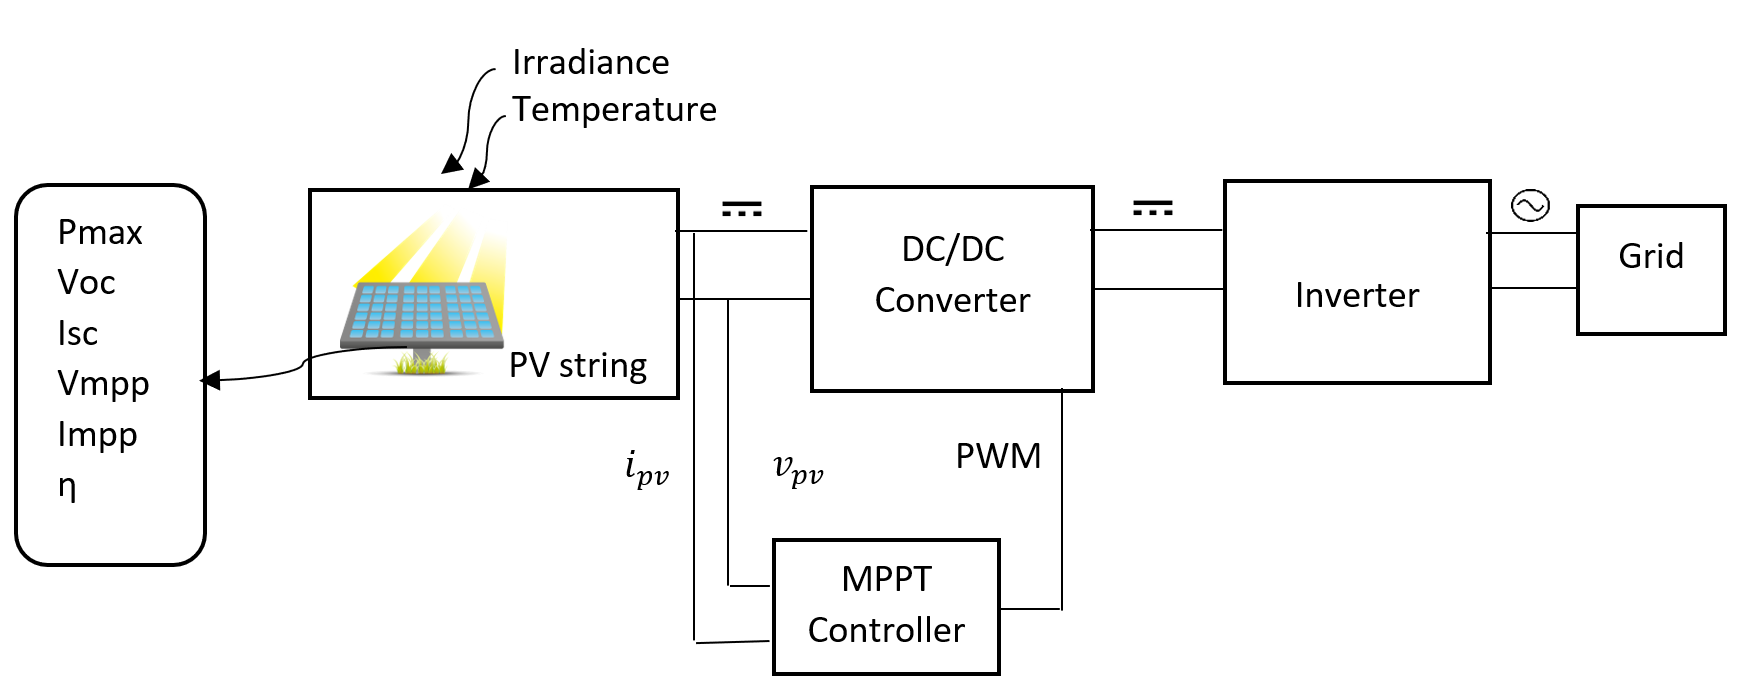
\includegraphics[width=\linewidth]{../Pictures/PV_system_blocks}
	\caption{Basic diagram of a PV system.}
	\label{fig:PVsystemblocks}
\end{figure}

HERE DESCRIPTION OF FIGURE IS MISSING. TYPES OF PV SYSTEMS: GRID-CONNECTED AND OFF-GRID
\newpage

\section{MIC implementation}
One of the most important factors to take into consideration when implementing photovoltaic (PV) modules is to obtain the maximum energy possible out of the available hardware, if this is not done, energy that should have been obtained will instead be lost. Since energy (E) is equal to power (P) over time (t), power must be maximized when the energy is being extracted. To achieve such goal a maximum power point tracker needs to be implemented, this is an electrical system that is always on the search of the location of the point where power extraction can be peaked. 
\begin{figure}[htbp]
	\begin{center}
	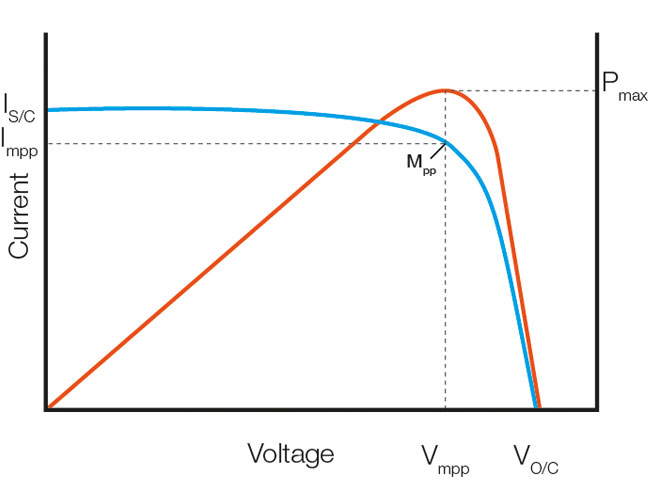
\includegraphics[width=0.7\linewidth]{../Pictures/mpp_graph.jpg}
	\caption{Maximum Power Point of generic solar panel.}
	\label{fig:mpp}
	\end{center}
\end{figure}

%[http://www.seaward-groupusa.com/userfiles/curve-tracing.php]%

MPPTs mostly consist on a power circuit that regulates either voltage drop or current flow across the PV terminals. There are many kinds of circuits that can be used to follow the maximum power point (MPP) of the PV, this topic will be further introduced in section blabla. 
However, solar plants and domestic used installations are composed of many modules, these modules are then connected to each other in series, parallel or in antiparallel configurations. To simplify the system, one MPPT is commonly used for many modules, this approach may lead to imperfections in the efficiency rates since the lower power generation of one module will then produce imperfections in the tracking system. 
This project focuses on the implementation of module integrated dc-dc converters (MICs). Using MICs for each module results in higher overall efficiencies, with this technology, events like partial shading, uneven dirt or wear distribution or imperfections produced in the assembly line are reduced and do not affect the rest of the modules in a line. Also, a more detailed control of the plant is achieved since separate data from each individual panel is obtained.
Different implementation options for MIC devices are possible but the most important objective of these devices is to individually control each module, resulting on an overall better efficiency rate, as well as a more robust system against any kind of inclemency. Each PV module will then be connected directly to each MIC, with this setup the output voltage and current are regulated by the device that extracts the energy, either an inverter, a battery or a load, allowing the system to work at different voltage and current levels whilst maintaining the MPP at all time.

\section{State of The Art}




